\documentclass[../ProgettoTecWeb2.tex]{subfiles}

\begin{document}
\section{L'homepage}
	\begin{figure} [H]
		\centering
		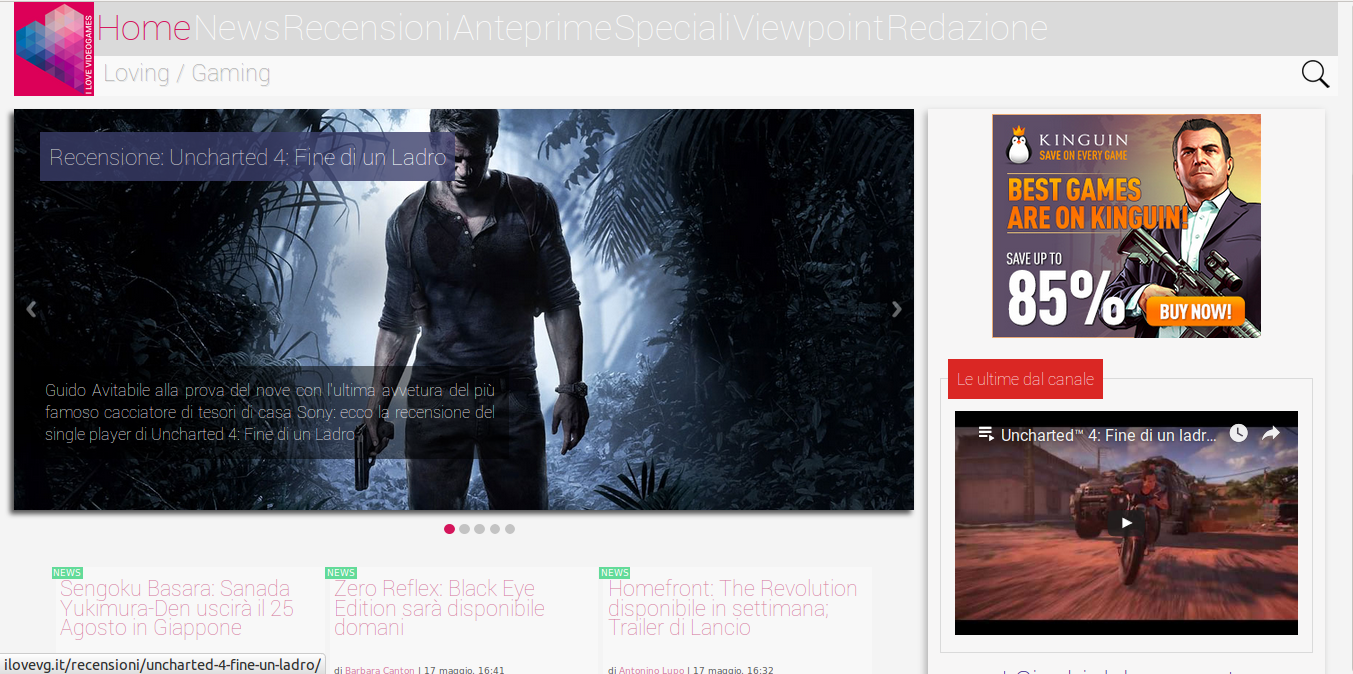
\includegraphics[scale=0.3]{img/ScreenHomePage}
		\caption{Homepage del sito}
	\end{figure}
	\subsection{Le 6W}
		L'homepage di un sito web dovrebbe sempre rispondere alle 6W giornalistiche, un po' riadattate al contesto del web.
		\subsubsection{Where}
			L'asse \textit{where} indica in che tipo di sito sono arrivato. Il primo impatto già ci fornisce indicazione sul contenuto del sito web difatti troviamo la prima pagina disseminata di immagini di videogiochi. Sotto il menù troviamo una grande scritte che recita \textit{Loving / Gaming} ed inoltre nella colonna a sinistra troviamo il link al canale youtube associato al sito web, che presenta video di gameplay, ed una lista dei giochi del momento. Anche la pubblicità in alto nella colonna di destra aiuta a capire il contesto poichè rimanda ad un altro sito web per la vendita di videogiochi.
		\subsubsection{Who}
			L'asse \textit{who} indica chi rappresenta il sito web. In alto a sinistra è possibile vedere il logo del sito web con vicino il nome. Tale logo segue il menu nel caso di scroll nella pagina e quindi è sempre visibile. Il nome forse è un po' troppo piccolo. Nel menù inoltre è presente il link per arrivare alla sezione \href{http://ilovevg.it/redazione/}{Redazione}. Tale sezione presenta in modo ironico le persone che collaborano al sito web e quindi a chi rappresenta realmente il sito.
		\subsubsection{Why}
			L'asse \textit{why} deve esporre i benefici del sito web. Come sopra citato il sito si occupa di recensioni e notizie riguardanti il mondo dei videogiochi. Tale asse è soddisfatto dalle scritte sopra le immagini che comprendono il tipo di contenuto(news, recensione, speciale o anteprima) seguito da un titolo e dai riquadri che contengono una anteprima di un contenuto(anch'essi espongono, nella parte superiore, il tipo di contenuto). L'asse è poi soddisfatto anche grazie al menu che comprende le voci:
			\begin{itemize}
				\item News;
				\item Recensioni;
				\item Anteprime;
				\item Speciali;
				\item Redazione.
			\end{itemize}
		\subsubsection{What}
			L'asse \textit{what} indica cosa il sito offre. Le offerte del sito web sono abbastanza evidenti: infatti subito si vedono le immagini relative alle notizie e recensioni principali. Scendendo nella pagina poi si possono vedere altre notizie e recensioni. Anche in questo caso l'identificazione di tale asse è semplificata dal menù.
		\subsubsection{When}
			L'asse \textit{when} indica le novità temporali relative al sito. Questo è l'asse sicuramente più evidente dato che è un sito che propone notizie e recensioni. È possibile notare, inoltre, come queste siano ordinate cronologicamente dall'alto al basso nella pagina.
		\subsubsection{How}
			L'asse \textit{how} ha il compito di indicare come arrivare alle sezioni principali del sito. Questo asse è risolto dal menù, che segue l'utente anche durante lo scroll nella prima pagina. Al di sotto del menù è presente la barra di ricerca, utile in un sito che comunque presenta molti contenuti.
			
	\subsection{Considerazioni generali}
		Nella parte alta della pagina è presente un riquadro con delle immagini che cambiano periodicamente, relative alle notizie principali, e con poco testo associato. Tali immagini andrebbero forse ridotte per dare più risalto a titoli e testo a loro associato.
		L'homepage del sito web è organizzata con una visualizzazione a griglia delle notizie in ordine cronologico. Tale organizzazione, anche se più compatta, è svantaggiosa per l'utente e comporta una maggiore fatica nella ricerca di una particolare notizia e quindi fa perdere più tempo.
		Inoltre tali notizie sono presentate con uno scroll infinito. Tale scelta è negativa poichè:
		\begin{itemize}
			\item un utente medio è disposto a scrollare per 1,3 schermi, per un totale quindi di 2,3 schermi: in questo modo possono essere perse molte delle notizie anche recenti;
			\item non rispetta i timer degli utenti: gli utenti in media passano 31 secondi nella prima pagina la prima volta che visitano il sito, che diminuisce nelle visite successive stabilizzandosi intorno ai 19 secondi. Ciò fa si che l'asse \textit{when} non possa essere soddisfatto a pieno visto che un utente difficilmente accedere a tutte le ultime notizie;
			\item lo scroll infinito nasconde il piè di pagina dove sono presenti il riferimento alla licenza per i contenuti presenti nel sito e i link con i quali è possibile accedere alle pagine collegate al sito dei maggiori social. 
		\end{itemize}
		In generale potrebbe essere preferibile spezzare tale scroll in più pagine. \\
		Un problema minore legato allo scroll infinito nella prima pagina è che viene visualizzato il simbolo del caricamento nell'attesa che vengano recuperati i contenuti successivi. Questa icona, sebbene possa ben adattarsi in un sito di videogiochi, nel caso di una connessione non perfetta, può essere fastidiosa perché fa si che venga ricordato continuamente all'utente che è in attesa.
		\begin{figure} [H]
			\centering
			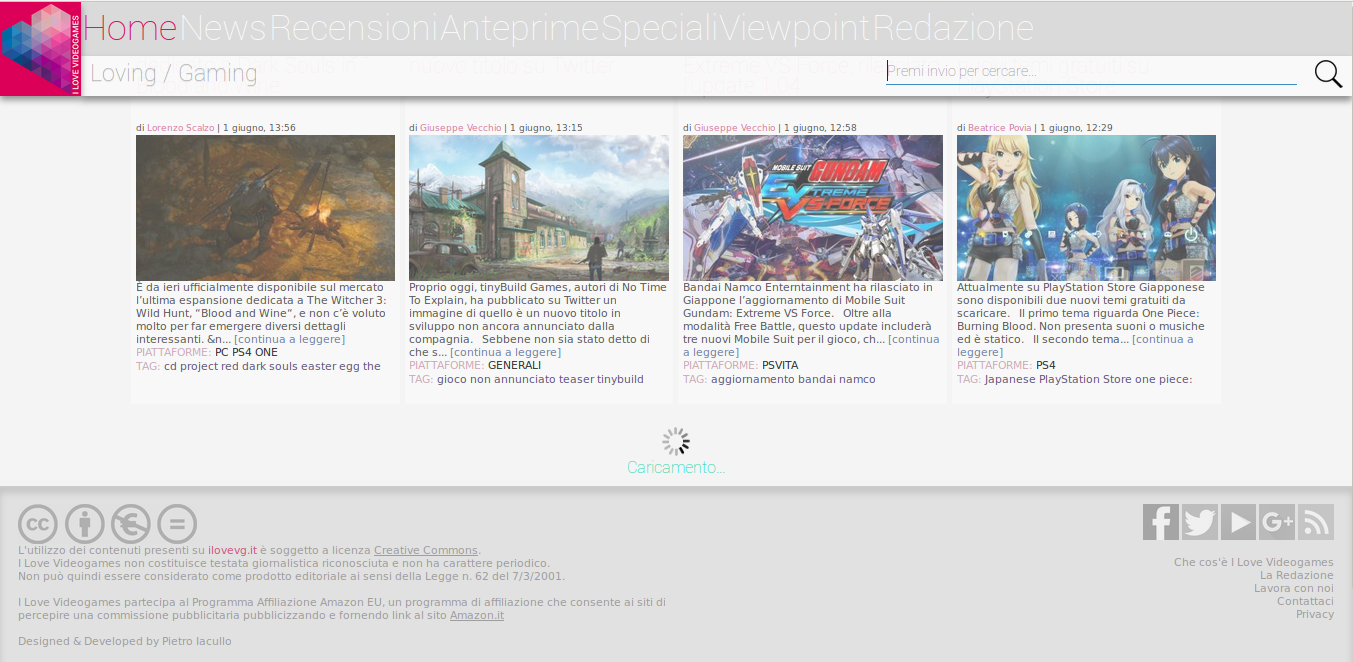
\includegraphics[scale=0.3]{img/PieDiPaginaHomepage}
			\caption{Piè di pagina dell'homepage}
		\end{figure}

		Il layout della prima pagina viene spezzato al di sotto della barra a destra che presenta della pubblicità e la classifica con i giochi del momento. Tale rottura fa si che, quando la barra non è più visibile, il contenuto venga ridimensionato e spostato al centro. Ciò può non essere gradevole per un utente che potrebbe non capire cosa è successo soprattutto nel caso in cui scrolli rapidamente. \\

		In conclusione sarebbe inoltre necessario dare maggior risalto al testo riportato: infatti nella prima pagina è dato molto risalto alle immagini relative alle notizie ma non uno spazio sufficiente, a mio parere, ai titoli e alle didascalie associate.

		\begin{figure} [H]
			\centering
			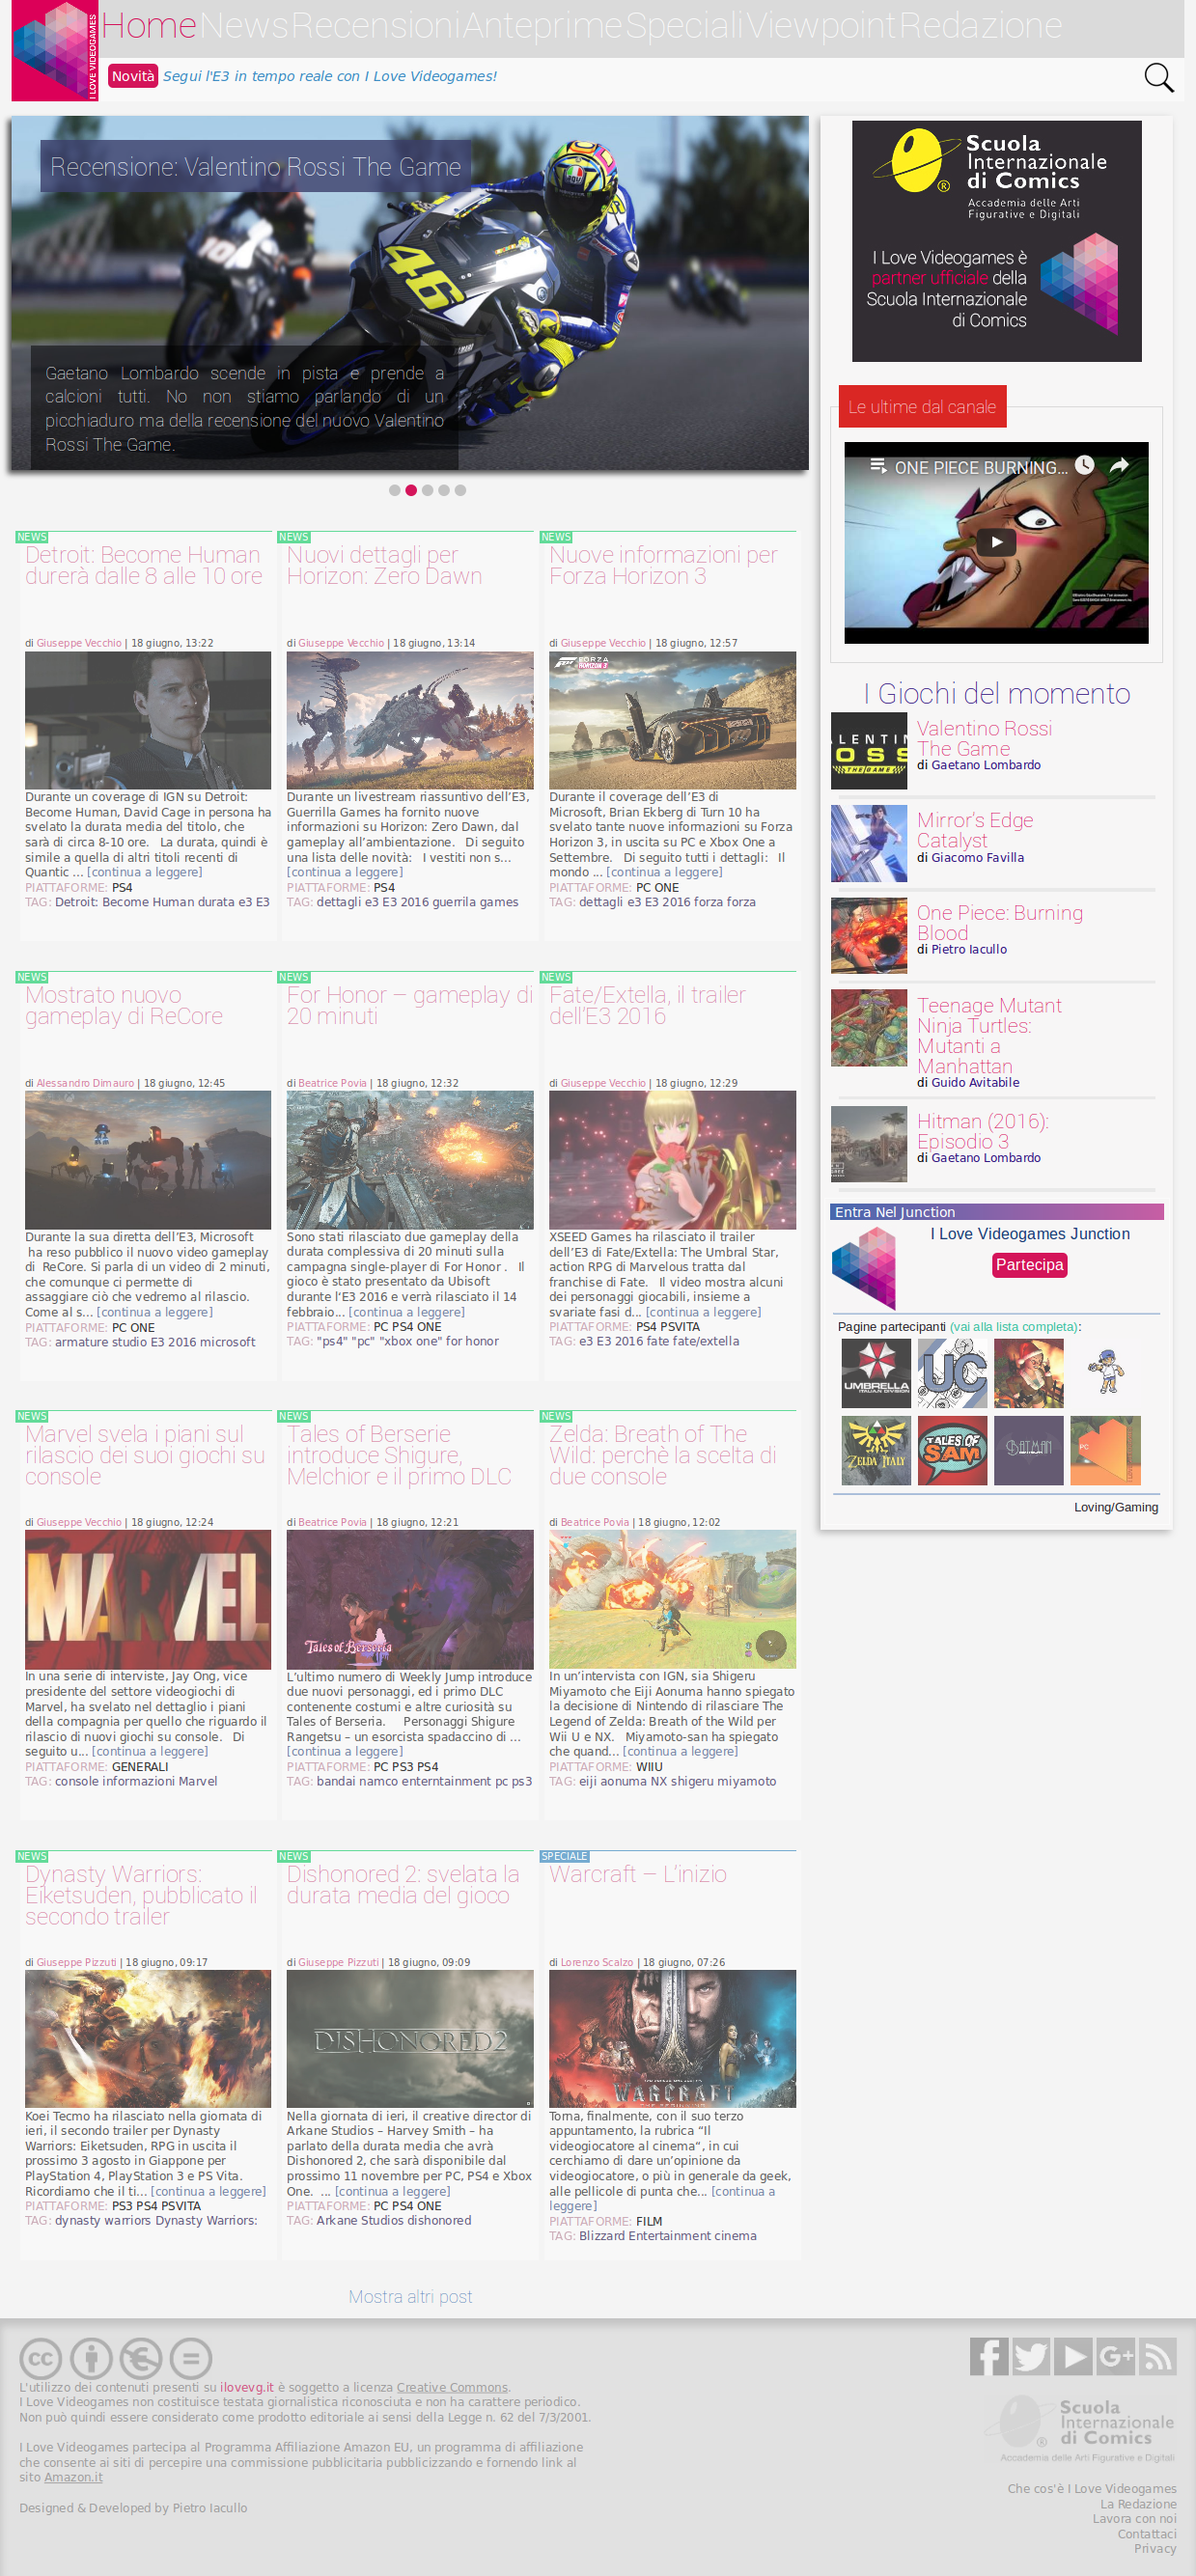
\includegraphics[scale=0.21]{img/HomePageCompleta}
			\caption{Home page completa del sito web}
		\end{figure}

\end{document}
